\documentclass[a0]{4by3}
\usepackage{braket}
\usepackage{multicol,graphicx,color}
\usepackage{amsmath,amssymb,amsthm}
\usepackage{tabularx}
\usepackage{mathrsfs}
\usepackage{mathtools}
\usepackage{caption}
\usepackage{xparse}
\usepackage{enumerate}
\usepackage{tikz}
\usetikzlibrary{arrows.meta}
\newtheorem{theorem}{Theorem}
\newtheorem{definition}{Definition}
\newtheorem{corollary}{Corollary}
\newtheorem{problem}{Problem}
\newtheorem{conjecture}{Conjecture}
\newtheorem{approach}{Approach}
\newtheorem{lemma}{Lemma}
\newtheorem{idea}{Idea}
\newtheorem*{prop}{Result}
\newtheorem*{cor}{Corollary}
\newcommand{\defeq}{\vcentcolon=}

%%%%%%%%%%%%%%%%%%%%%%%%%%%%%%%%%%%%
% VARIABLES & LAYOUT CONFIGURATION %
%%%%%%%%%%%%%%%%%%%%%%%%%%%%%%%%%%%%

% Colors
%%%% THIS IS WHERE YOU CAN CHANGE COLORS. 
\definecolor{titlebackground}{rgb}{0.0, 0.0, 0.5}
\definecolor{titletext}{rgb}{1, 1, 1}
\definecolor{titlesubtext}{rgb}{0.52, 0.586, 0.664}
\definecolor{subtitleoutline}{rgb}{0.0, 0.0, 0.5}
\definecolor{subtitlebackground}{rgb}{0.86, 0.84, 0.82}
\definecolor{subtitletext}{rgb}{0.0, 0.0, 0.5}
% Colors

% Columns
%%%% THIS IS WHERE YOU CAN CHANGE THE HEIGHT & NUMBER OF COLUMNS
\newcommand{\ColumnScale}{0.74526}
\newcommand{\NumColumns}{4}
\setlength{\fboxsep}{1cm}
\setlength{\columnsep}{3cm}
\color{titlesubtext}
\setlength{\columnseprule}{2mm}
\setlength{\fboxsep}{1cm}
\setlength{\fboxrule}{5mm}
% Columns

% Font Helvetica
\renewcommand\sfdefault{phv}
\renewcommand\familydefault{\sfdefault}
% Font Helvetica

% Math
\setlength{\abovedisplayskip}{5pt}
\setlength{\belowdisplayskip}{5pt}
% Math

%%%%%%%%%%%%%%%%%%%%%%%%%%%%%%%%%%%%
% FANCY COMMANDS                   %
%%%%%%%%%%%%%%%%%%%%%%%%%%%%%%%%%%%%

% Create the fancy title command
\NewDocumentCommand{\FancyTitle}{ O{1.25cm} m m m }{
    \noindent
    \colorbox{titlebackground}{\begin{minipage}{\dimexpr\textwidth+\fboxsep+2\fboxrule\relax-2\fboxsep}
      \begin{center}\vspace{5mm}
       {\VeryHuge \textcolor{titletext}{#2}}\\[10mm]
       {\Huge \textcolor{titletext} {#3}}\\[10mm]
       {\Large \textcolor{titletext}{#4}}
      \end{center}
    \end{minipage}}
    \vspace{#1}
}

% Create the fancy subtitle command
\NewDocumentCommand{\FancySubtitle}{ O{1cm} O{1cm} m }{
    \vspace{#2}
    \noindent
    \fcolorbox{subtitleoutline}{subtitlebackground}{\begin{minipage}{\dimexpr\linewidth-2\fboxsep-2\fboxrule\relax}
        \centering
        \sf \huge \textcolor{subtitletext}{#3}
    \end{minipage}}
    \vspace{#1}
}

% Create the fancy figure command
\NewDocumentCommand{\FancyFigure}{ O{0.9} m m m }{
    \begin{center}
        \begin{minipage}{#1\linewidth}
          \centering
          \includegraphics[width=\linewidth]{#2}
          \captionof{figure}{#3}
          \label{#4}
        \end{minipage}
    \end{center}
}

%%%%%%%%%%%%%%%%%%%%%%%%%%%%%%%%%%%%

\begin{document}

\FancyTitle{A catchy, very cool title:}{A subtitle if you want it}{Names of all the important people who contributed, i.e. everyone in the group}

%Main
\color{black}
\noindent
\begin{minipage}{\linewidth + 2\fboxsep}
\begin{multicols*}{\NumColumns}
    \FancySubtitle[5mm]{Overview}
        \begin{center}
          \includegraphics[width=1\linewidth,trim={0 9cm 0 11cm},clip]{a_picture if you want it.png}
        \end{center}
        
        \large
       This is where you can put an abstract/brief description of the project

Keep in mind that you want the font size to be relatively large to make readability a maximum.



    \FancySubtitle[0cm][2cm]{The problem}
    
        \begin{center}
        \LARGE{\textbf{Assumptions \& Equations}}
        \end{center}
        \vspace{5mm}
            \large
        
            

As the sun dipped below the horizon, casting hues of orange and pink across the sky, the quaint village came to life with the soft chatter of its inhabitants. Children chased each other through narrow cobblestone streets, their laughter echoing against the ancient stone walls. The scent of freshly baked bread wafted from the local bakery, enticing passersby with its warm embrace. In the distance, the sound of church bells rang out, signaling the end of another peaceful day in this idyllic countryside retreat.


As the sun dipped below the horizon, casting hues of orange and pink across the sky, the quaint village came to life with the soft chatter of its inhabitants. Children chased each other through narrow cobblestone streets, their laughter echoing against the ancient stone walls. The scent of freshly baked bread wafted from the local bakery, enticing passersby with its warm embrace. In the distance, the sound of church bells rang out, signaling the end of another peaceful day in this idyllic countryside retreat.










As the sun dipped below the horizon, casting hues of orange and pink across the sky, the quaint village came to life with the soft chatter of its inhabitants. Children chased each other through narrow cobblestone streets, their laughter echoing against the ancient stone walls. The scent of freshly baked bread wafted from the local bakery, enticing passersby with its warm embrace. In the distance, the sound of church bells rang out, signaling the end of another peaceful day in this idyllic countryside retreat.



            \columnbreak
            You could use Tikz to make figures (if you want)
            
            \begin{center}
                \vspace{5mm}
                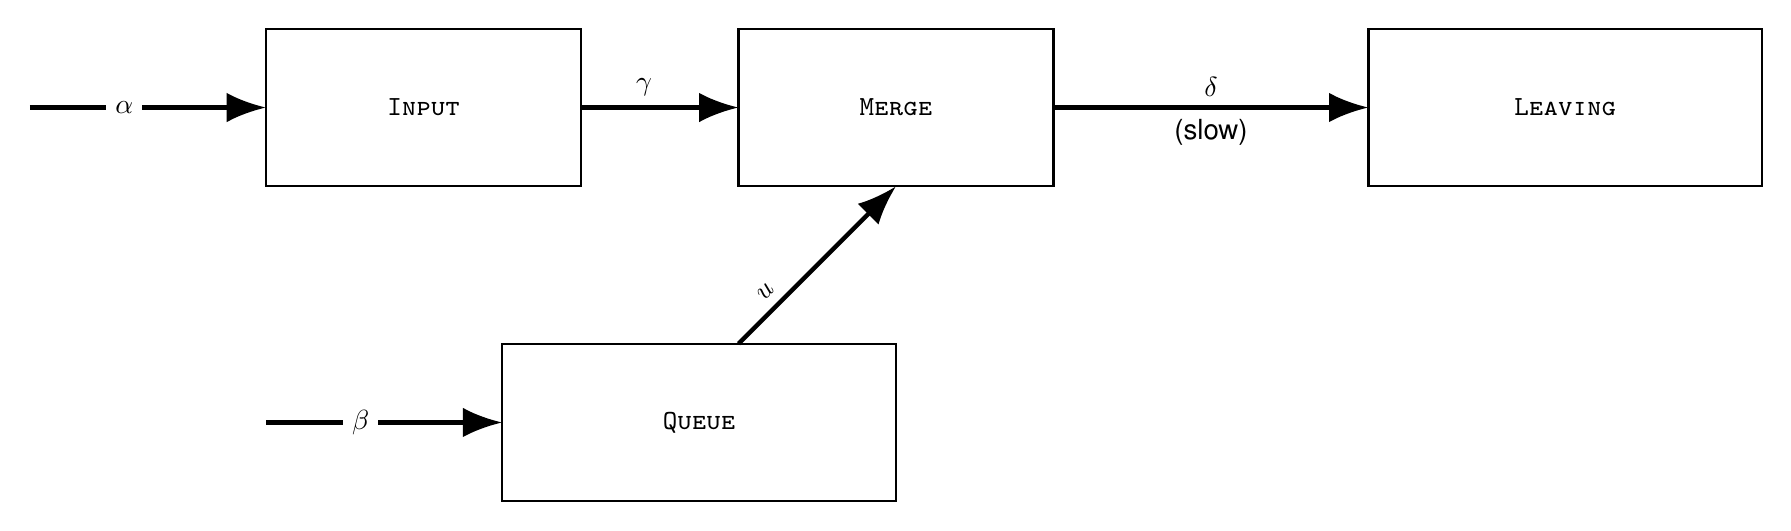
\begin{tikzpicture}
                    \draw[thick] (0,0) rectangle ++(4,2) node[midway] {\textsc{\texttt{Input}}};
                    \draw[thick] (6,0) rectangle ++(4,2) node[midway] {\textsc{\texttt{Merge}}};
                    \draw[thick] (14,0) rectangle ++(5,2) node[midway] {\textsc{\texttt{Leaving}}};
                    \draw[thick] (3,-4) rectangle ++(5,2) node[midway] {\textsc{\texttt{Queue}}};
                    \draw[-{Latex[length=5mm]}, ultra thick] (-3, 1) -- (0, 1) node[pos=.4, fill=white] {$\alpha$};
                    \draw[-{Latex[length=5mm]}, ultra thick] (0, -3) -- (3, -3) node[pos=.4, fill=white] {$\beta$};
                    \draw[-{Latex[length=5mm]}, ultra thick] (4, 1) -- (6, 1) node[pos=.4,above] {$\gamma$};
                    \draw[-{Latex[length=5mm]}, ultra thick] (10, 1) -- (14, 1) node[midway,above] {$\delta$} node[midway,below] {(slow)};
                    \draw[-{Latex[length=5mm]}, ultra thick] (6,-2) -- (8,0) node[near start,sloped,above] {$u$};
                \end{tikzpicture}
                \vspace{5mm}
            \end{center}
        
        \begin{center}
        \LARGE{\textbf{The approach}}
        \end{center}
            \large
        
            Describe what you are going to try and accomplish
	As the sun dipped below the horizon, casting hues of orange and pink across the sky, the quaint village came to life with the soft chatter of its inhabitants. Children chased each other through narrow cobblestone streets, their laughter echoing against the ancient stone walls. The scent of freshly baked bread wafted from the local bakery, enticing passersby with its warm embrace. In the distance, the sound of church bells rang out, signaling the end of another peaceful day in this idyllic countryside retreat.


            
            \FancyFigure{Figure file}{Figure caption.}{fig:evolution-comparison}
        
        \begin{center}
        \vspace{2cm}
        \LARGE{\textbf{Another heading}}
        \end{center}
            \large
        
            As the sun dipped below the horizon, casting hues of orange and pink across the sky, the quaint village came to life with the soft chatter of its inhabitants. Children chased each other through narrow cobblestone streets, their laughter echoing against the ancient stone walls. The scent of freshly baked bread wafted from the local bakery, enticing passersby with its warm embrace. In the distance, the sound of church bells rang out, signaling the end of another peaceful day in this idyllic countryside retreat.


        \columnbreak
        \begin{center}
        \LARGE{\textbf{Infinite-Time LQR}}
        \end{center}

            Only if you actually used Infinite-Time LQR?
As the sun dipped below the horizon, casting hues of orange and pink across the sky, the quaint village came to life with the soft chatter of its inhabitants. Children chased each other through narrow cobblestone streets, their laughter echoing against the ancient stone walls. The scent of freshly baked bread wafted from the local bakery, enticing passersby with its warm embrace. In the distance, the sound of church bells rang out, signaling the end of another peaceful day in this idyllic countryside retreat.


    \FancySubtitle[4mm][1cm]{Early Results \& Analysis}
    
        \begin{center}
          \includegraphics[width=1\linewidth,trim={0 8cm 0 10cm},clip]{anothepicture.png}
        \end{center}
        
        As the sun dipped below the horizon, casting hues of orange and pink across the sky, the quaint village came to life with the soft chatter of its inhabitants. Children chased each other through narrow cobblestone streets, their laughter echoing against the ancient stone walls. The scent of freshly baked bread wafted from the local bakery, enticing passersby with its warm embrace. In the distance, the sound of church bells rang out, signaling the end of another peaceful day in this idyllic countryside retreat.

As the sun dipped below the horizon, casting hues of orange and pink across the sky, the quaint village came to life with the soft chatter of its inhabitants. Children chased each other through narrow cobblestone streets, their laughter echoing against the ancient stone walls. The scent of freshly baked bread wafted from the local bakery, enticing passersby with its warm embrace. In the distance, the sound of church bells rang out, signaling the end of another peaceful day in this idyllic countryside retreat.

          \columnbreak  
 As the sun dipped below the horizon, casting hues of orange and pink across the sky, the quaint village came to life with the soft chatter of its inhabitants. Children chased each other through narrow cobblestone streets, their laughter echoing against the ancient stone walls. The scent of freshly baked bread wafted from the local bakery, enticing passersby with its warm embrace. In the distance, the sound of church bells rang out, signaling the end of another peaceful day in this idyllic countryside retreat.

   \FancySubtitle[4mm][1cm]{Conclusions and next steps}
  As the sun dipped below the horizon, casting hues of orange and pink across the sky, the quaint village came to life with the soft chatter of its inhabitants. Children chased each other through narrow cobblestone streets, their laughter echoing against the ancient stone walls. The scent of freshly baked bread wafted from the local bakery, enticing passersby with its warm embrace. In the distance, the sound of church bells rang out, signaling the end of another peaceful day in this idyllic countryside retreat.
 As the sun dipped below the horizon, casting hues of orange and pink across the sky, the quaint village came to life with the soft chatter of its inhabitants. Children chased each other through narrow cobblestone streets, their laughter echoing against the ancient stone walls. The scent of freshly baked bread wafted from the local bakery, enticing passersby with its warm embrace. In the distance, the sound of church bells rang out, signaling the end of another peaceful day in this idyllic countryside retreat.

    \bibliographystyle{amsalpha}
    \bibliography{poster_references}
\end{multicols*}
\end{minipage}

\nocite{unsplash}
%Using nocite allows a reference to appear in the reference list without a citation appearing in the poster.
\footnotesize

\end{document}